\documentclass[12pt]{article}
\usepackage[francais]{babel}
\usepackage[utf8]{inputenc}
\usepackage[top=35mm, bottom=35mm, left=25mm, right=25mm]{geometry} 
\usepackage[T1]{fontenc} 
\usepackage{geometry}
\usepackage{graphicx}
\usepackage{multirow}  
\usepackage{subfigure}
\usepackage{verbatim}
\usepackage{url}
\usepackage{algorithmic, algorithm} 
\usepackage{amsmath,amsfonts,amssymb}
\usepackage{lmodern}
\usepackage{microtype}
\usepackage{xcolor}
\usepackage{textcomp}
\usepackage{hyperref}
\usepackage{listings}
\usepackage{color}

\hypersetup{
    colorlinks,
    citecolor=blue,
    filecolor=black,
    linkcolor=magenta,
    urlcolor=blue,
}

\hypersetup{
pdftitle={Rapport de Graphe},
pdfsubject={Compte-rendu du projet de graphe},
pdfauthor={LEPAGE Guillaume},
pdfkeywords = {Graphes, Université de Limoges, Faculté des Sciences et Techniques}
}
\setcounter{secnumdepth}{3}
\usepackage{fancyhdr}
\pagestyle{fancy}
 \lhead{\leftmark}
 \rhead{}
 
\begin{document}

\begin{titlepage}
\setlength{\headheight}{0cm}
\setlength{\headsep}{0cm}
{

  \begin{center}
    { \small \textsc{Université de Limoges}\\
      \textsc{Faculté des Sciences et Techniques}\\
    }

    \vspace{2cm}

      \textbf {	Année Universitaire 2015 - 2016\\
      			version du 15 mai 2016}
    \vspace{2cm}  

    \fbox{ 
      \begin{minipage}[h]{.9\linewidth}
        \begin{center}
          {\vspace*{5mm}
           \huge\textbf{Rapport de Graphe}\\
            \vspace*{5mm}}
        \end{center}
      \end{minipage}
    }

    \vspace{15mm}

    Auteurs\\~\\
    {\large 
    \bsc Etienne BOESPFLUG\\
    	 Guillaume LEPAGE}\\
    ~\\
   \underline{Licence \textsc{Informatique}, semestre 6}\\ 

	\vspace{3cm}  

  \begin{figure}[!h]
	\centering
	
\includegraphics[height=25mm]{imgs/unilim-fst.jpg}
  \end{figure}
  \end{center}
  
  \vfill
  \begin{flushleft}
	Responsable Travaux Pratiques : Jean-Christophe \bsc{Deneuville}\\
	Responsable Module Graphes : Philippe \bsc{Gaborit}\\
\end{flushleft}
  }
\end{titlepage}

\newpage		
\tableofcontents
\addcontentsline{toc}{section}{Table des matières}

\clearpage 

% CONTENT

\section{Architecture générale}
Un graphe se défini par un ensemble de sommets et d'arêtes. 
\subsection{Graphe orientés et non-orientés}
Dans notre implémentation, nous avons fait le choix de considérer tous les graphes comme orientés. \\
\\
En effet, un graphe non-orienté est un graphe orienté qui dispose d'une arêtes (x, y) pour chaque arête (y, x). Dans le cas d'un graphe pondéré, la valeur de l'arête (x, y) est alors la même que celle de l'arête (y, x). De cette manière, les arêtes (x, y) et (y, x) correspondent à l'arc (x; y) d'un graphe non-orienté.\\ 

Cela permet de manipuler indifféremment des graphes orientés et non-orientés et possiblement de faire évoluer la nature du graphe en ajoutant/supprimant des arêtes. \\ 

Étant donné que certains des algorithmes demandés pour le projet ne s'appliquent que pour des graphes non-orientés ({\bf Kruskal} et {\bf Prim} notamment), nous avons ajouté des fonctions permettant de vérifier si un graphe est ou non orienté.\\ 

En compensation de la flexibilité de ce choix de conception, il est nécessaire d'effectuer une vérification de la nature du graphe et de ne manipuler qu'une arête sur deux lorsqu'on souhaite manipuler un graphe qu'on sait non-orienté, ce qui ajoute un surcoût de calcul. \\ 

\clearpage
\subsection{Structures Standards:}
Différentes structures de données permettent de représenter un graphe. Chacune d'entre elles dispose d'avantages spécifiques, que ce soit en terme de vitesse d'accès à certaines données, de taille mémoire ou de flexibilité :\\  \begin{itemize}
\item Matrice d'adjacence : On associe au graphe une matrice de taille |V|² (où |V| est le nombre de sommets du graphe) de booléens. Les sommets sont implicitement stockés (ils correspondent aux indexes de la matrices). m(i, j) = vrai, s'il existe une arête (i, j). 
Le nombre de successeurs ou de prédécesseurs se calcule facilement en parcourant les lignes et les colonnes de la matrice.\\
\item Matrice d'incidence : Cette structure n'est applicable qu'aux graphes sans boucles. La taille en mémoire est inférieure à celle de la matrice d'adjacence si le nombre d'arêtes est inférieur au nombre de nœuds puisque la matrice est de taille |E| x |U| (avec |E| le nombre de nœuds et |U| le nombre d'arêtes).\\
\item Liste d'adjacence : la liste d'adjacence fait partie des moins gourmandes en mémoire (|E| + |U|) mais peut présenter des performances moindre lors de l'insertion d'arêtes (il faut utiliser une liste chaînée pour faciliter l'insertion en milieu de liste) et de sommets (ajouter un sommet demande de recalculer les indexes du début des arêtes correspondantes).\\
\item Tableau d'entier : d'une taille de |U| + 1, cette structure stocke une liste d'entier correspondant aux identifiants des arêtes présentes. Une arête est alors identifiée par a = extrémité\char`_initiale * E + extrémité\char`_finale.\\
\item Le "Graphe informatique" : le graphe est représenté par un ensemble de structure Nœud. Chacun des nœuds stocke les arêtes incidentes (peut également stocker les arêtes sortantes pour améliorer les performances de calculs en dépit d'une place mémoire supérieure).
Cette structure est lourde en mémoire mais très flexible (on peut facilement pondérer le graphe ou ajouter une donnée aux sommets). \\
\end{itemize}

Cette liste n'est pas exhaustive et un grand nombre de variantes existe. Il n'y a pas une structure supérieure aux autres, chacune d'entre elles présentant des avantages et des inconvénients en fonction du contexte d'utilisation.

\clearpage
\subsection{Données des arêtes et des sommets}

En pratique, il est souvent nécessaire d'associer une donnée aux arêtes et aux nœuds. \\  \\
Pour un réseau social par exemple, les sommets sont des comptes utilisateurs. Pour un logiciel de calcul de trajets routiers, les nœuds sont des villes ou des carrefours et les arêtes sont des routes ou au moins des distances.\\ \\
Parmi les algorithmes demandés, ceux permettant le calcul des plus courts chemins ({\bf Djikstra} et {\bf Bellman-Ford}) nécessitent un graphe pondéré (et donc un type de valeur pour les arêtes).\\

\subsection{Le choix d'une structure paramétrable}
La structure de donnée idéale étant dépendante du contexte, nous avons choisi d'utiliser une structure paramétrée statiquement. \\ 

Notre implémentation tire profit des templates C++ pour permettre au code client de choisir la structure de donnée de base à utiliser et le type de valeur des arêtes. Les algorithmes sont ainsi applicables à des graphes basiques ou comportant une pondération d'un type défini. Nous n'avons pas fourni la possibilité de paramétrer le graphe avec un type associés au sommet puisque cela n'était utilisé dans aucun des algorithmes demandés mais cela peut se faire simplement en utilisant la même méthode.  \\ 

Dans le rendu, deux structures de données basiques sont disponibles : {\it AdjacencyMatrixModel} : matrice d'adjacence, et {\it AdjacencyListModel} : liste d'adjacence. La classe {\it Graph} est paramétrée par une structure basique et un type pour les arêtes permettant de représenter des graphes pondéré ou non (le type {\it void} est utilisé par défaut et signifie que le graphe n'est pas pondéré).  \\ 

Une autre solution aurait été d'utiliser le polymorphisme pour permettre un changement dynamique de la structure interne du {\it graphe}. De cette manière, on pourrait à tout moment utiliser la structure de donnée la plus adaptée. Néanmoins, le changement de structure a un coût non négligeable et déterminer sous quelles conditions ce coût est acceptable demanderait de faire une analyse poussée (en plus d'être dépendant du contexte d'utilisation de la structure). \\ 

Ainsi, nous définissons une interface de base pour une structure de donnée représentant un graphe orienté non-pondéré ce qui nous permet ensuite d'appliquer les algorithmes (et d'étendre la structure à des graphes pondérés) indépendamment de la structure interne spécifiée. \\ 

La spécialisation template permet également d'effectuer des optimisations lorsqu'une structure de donnée spécifique est utilisée, et que celle-ci a des facilités d'accès à certaines informations. Nous n'avons évidemment pas fait toutes les optimisations possibles mais notre architecture permettrait à quelqu'un qui souhaiterait améliorer les cas spécifiques de le faire sans modifier le code client. \\ 

\section{Précisions sur les sources rendues }
Vous trouverez dans l'archive rendue l'intégralité des fichiers sources (.cpp) et des headers (.h / .tpp). Le programme a été développé en C++ standard (C++14 : ISO/CEI 14882:2014) et nécessite donc d'être compilé avec un compilateur supportant la norme C++14.\\ \\
Les classes et les fonctions utilisées pour la manipulation des graphes sont contenues dans l'espace de nom {\it graph}. \\ \\
Les pré-conditions des fonctions sont vérifiées avec la macro standard {\it assert}. Des exceptions sont levées uniquement lorsque des fichiers ne sont pas trouvés (lors de la lecture et la sauvegarde d'un graphe). \\ 

 En l'état actuel, le programme lance quelques fonctions d'exemple permettant d'exécuter les algorithmes demandés sur des graphes prédéterminés (dont les données sont stockées dans des fichiers présent dans l'archives à l'extension .g). Pour n'exécuter que certains exemples, il vous suffit de mettre en commentaire dans la fonction main les appels de fonctions concernant les exemples qui ne vous intéressent pas. \\ 
 
 \clearpage
 
 L'interface commune aux types utilisés comme des graphes est composées des entités suivantes : \\ \begin{itemize}
\item vertex\_t : le type utilisé pour identifier un sommet. Il est utilisé d'une manière semblable aux itérateurs de la STL ({\bf S}tandard {\bf T}emplate {\bf L}ibrary), il s'agit du type {\it size\_t} pour les différents types disponibles dans notre implémentation.
\item edge\_t : le type utilisé pour identifier une arête. Il s'agit également du type {\it size\_t} pour tous les types fournis.
\item constructeur par défaut : permet l'instanciation d'un graphe sans sommet. Cela n'est utile que si on décide par la suite d'autoriser la suppression/ajout de sommets.
\item constructeur prenant en entrée le nombre de sommet ({\it size\_t}) : permet l'instanciation d'un graphe avec un nombre défini de sommets.
\item bool isDirected() const : renvoie vrai si le graphe est orienté, faux sinon.
\item edge\_t edge(vertex\_t, vertex\_t) const : renvoie l'identifiant de l'arête ayant pour origine le premier sommet passé en paramètre et le second comme sommet d'arrivée.
\item bool existVertex(vertex\_t) const: renvoie vrai si le sommet passé en paramètre est présent dans le graphe.
\item bool existEdge(edge\_t) const : renvoie vrai si l'arête passée en paramètre est présente dans le graphe. L'identifiant passé doit être valide.
\item size\_t vertexCount() const : renvoie le nombre de sommets du graphe.
\item size\_t edgeCount() const : renvoie le nombre d'arêtes du graphe.
\item std$::$pair<size\_t, size\_t> size()  const : renvoie la paire (nombre de sommet, nombre d'arêtes).
\item vertex\_t begin() : renvoie l'identifiant sur le premier sommet du graphe.
\item vertex\_t end() : renvoie l'identifiant suivant le dernier sommet du graphe.
\item vertex\_t cbegin() const et vertex\_t cend() const : même utilisation que leurs homologues non constants. Il s'agit simplement de prévoir une éventuelle amélioration des identifiants pour en faire de véritable itérateurs (et donc de fournir des version const et non-const pour ne pas affecter le code client).
\item void removeEdge(edge\_t) : supprime l'arête du graphe (et sa valeur si le graphe est pondéré). Si l'arête n'existe pas, ne fait rien. \\
\end{itemize}
Interface spécifique aux graphes non-pondérés. Cela comprend les structures de données basiques ({\it AdjacencyMatrixModel}, {\it AdjacencyListModel}) et {\it Graph<void, T>}: \\ \begin{itemize}
\item void addEdge(edge\_t) : ajoute l'arête au graphe. Si l'arête existe déjà, ne fait rien.
\item Interface spécifique aux graphes pondérés (ici par le type indéfini EdgeData) :
\item void addEdge(edge\_t, EdgeData) : ajoute l'arête au graphe avec sa valeur. Si l'arête existe déjà, sa valeur est remplacée. 
\end{itemize}

\clearpage

\section{Parcours des graphes et composantes connexes}
\subsection{Parcours des graphes}
Nous avons implémenté les deux types de parcours de graphe, à savoir le parcours en largeur, et le parcours en profondeur. \\
Le parcours en largeur explore d'abord le sommet d'origine, puis les successeurs (ou voisins dans le cas d'un graphe non-orienté) de celui-ci, puis les successeurs non explorés de ceux-ci etc... \\
 À l'inverse, le parcours en profondeur consiste en une approche intuitivement récursive. Il va d'abord explorer le premier successeur non-exploré du sommet d'origine, puis le premier successeur de ce successeur etc… jusqu'à atteindre un sommet qui ne possède plus de successeurs non-exploré. Il va ensuite remonter les sommets explorés et prendre un second sommet non exploré, et ainsi de suite jusqu'à n'avoir plus aucun sommet explorés qui possède de successeurs non explorés.\\
Il est possible de passer une fonction de la forme {\it void(ItérateurSommet)} qui sera exécutée pour chaque sommet lors du parcours. Notez qu'il aurait pu être intéressant d'offrir la possibilité d'ajouter des arguments à cette fonction (cela nous aurait notamment permis d'utiliser les fonctions de parcours pour d'autres algorithmes).\\
\subsection{Composantes connexes}
Le calcul des composantes (fortement-)connexes se fait avec un unique algorithme. En effet, puisque les graphes non-orientés sont traités comme des graphes orientés avec simplement deux arêtes pour un arc, le calcul de la composante fortement connexe revient au calcul de la composante connexe pour un graphe non-orienté. \\
Les fonctions {\it stronglyConnectedComponents} et {\it isStronglyConnected} traitent donc la connexité simple (et non forte) si on considère un graphe comme étant non-orienté. \\
Notez que dans la suite de ce rapport, lorsque nous parlerons indifféremment de graphe orienté ou non-orienté (qui sont donc dans tous les cas représenté comme des graphes orienté), nous parlerons donc de composante fortement connexe, que le graphe soit orienté ou non.\\
\clearpage
\subsection{Exemples :}
Nous utilisons le graphe orienté suivant, contenu dans le fichier {\it "basicGraph.g"} afin d'afficher ses composantes fortement connexes ainsi qu'un parcours en profondeur qui affiche à chaque fois les successeurs du sommet : \\

\section{Sauvegarde et lecture de graphes}
Le format de fichier est le même pour les graphes pondérés et non pondérés. Celui-ci suit les règles de grammaire suivant : \\

S $::=$ $<$NOMBRE\_SOMMET$><$LISTE\_ARÊTES$>$ \\
$<$NOMBRE\_SOMMET$>$ $::=$ entier \\
$<$LISTE\_ARÊTES$>$ $::=$ $<$ARÊTE$><$LISTE\_ARÊTES$>$ | epsilon \\
$<$ARÊTE$>$ $::=$ $<$SOMMET$><$SOMMET$><$TYPE$>$  \\
$<$SOMMET$>$ $::=$ entier \\
$<$TYPE$>$ $::=$ suite de bit \\

Le fichier débute par le nombre de sommets que comporte le graphe, suivi par la liste des arêtes. Chaque arête est définie par le numéro du sommet de départ et d'arrivée, ainsi que la valeur associée à l'arête.\\ 

Cette valeur dépend donc de la pondération du graphe. Si le graphe est non pondéré, <TYPE> $::=$ epsilon. \\ 

Pour pouvoir être lu et sauvegardé dans un fichier texte, le graphe doit être pondéré par un type qui surcharge les opérateurs $>>$ et $<<$ pour les flux std$::$fstream (ou par {\it void} dans le cas d'un graphe non pondéré).\\ 

Dans les graphes utilisés pour les exemples d'exécution des algorithmes, les types utilisés sont {\it void} (graphe non-pondérés), {\it unsigned} ou {\it int}.\\ 

Nous avons choisi de ne pas ajouter d'informations aux graphes tels qu'un nom ou un identifiant puisque le code client peut créer une classe englobante s'il le souhaite.\\ 

\clearpage
\section{Arbre couvrant de poids minimum}

\subsection{Kruskal}
\subsubsection{L'algorithme :}

L'algorithme de {\bf Kurskal} permet de déterminer l'arbre couvrant de poids minimum à un graphe G connexe\footnote{En réalité, il est possible d'appliquer {\bf Kurskal} (et de fait {\bf Prim}) sur un graphe qui n'est pas connexe. Le résultat sera alors l'arbre couvrant minimum d'une des composantes connexes du graphe. La composantes en question dépends du sommet de départ qui a été choisi pour l'algorithme (et qui dépends de l'implémentation).
Dans notre implémentation, l'application de {\bf Kurskal} (et {\bf Prim}) sur un graphe non-connexe n'est pas autorisée.
}, pondéré et non-orienté. L'arbre couvrant minimum est l'arbre (graphe non-orienté, connexe et acyclique) dont la somme du poids de chaque arête est la minimum possible (et qui contient tous les sommets de G). \\ 

Puisque notre implémentation considère tous les graphes comme des graphes connexes, la première étape consiste à faire un tri dans les arêtes (puisqu'on considère ici les arêtes comme des arcs, il ne faut pas traiter deux fois le même arc). \\ 

Les arêtes (arcs) sont alors triés\footnote{En fonction de l'implémentation de la STL utilisée, l'algorithme de tri est diffèrent. Les algorithmes utilisés sont en général quicksort, heapsort ou encore introsort pour les implémentations modernes.} en fonction de leur poids (dans l'ordre croissant).\\ 

Un arbre contenant autant de sommets que le graphe d'entrée est créé. On a choisi de retourner un arbre non pondéré ici (la structure utilisée est la même que la structure interne utilisée par le graphe pondéré passé en paramètres) ainsi que le poids total. On aurait également pu choisir de retourner un arbre pondéré mais puisque les arêtes et les sommets présents dans l'arbre sont directement associées (par leurs identifiants {\it vertex\_t} et {\it edge\_t}) à ceux du graphe d'entrée ce n'était pas indispensable.\\ 

Ensuite, une boucle qui s'arrête lorsque l'arbre est connexe est démarrée. A chaque tour de boucle on ajoute l'arête de poids minimum qui ne forme pas de cycle. Pour détecter si l'ajout va créer un cycle, il faut vérifier que les deux sommets de l'arête sont situés dans des composantes connexes différentes.\\ 

\clearpage
\subsubsection{Exemple :}
Le programme main exécute l'algorithme de {\bf Kurskal} sur le graphe contenu dans fichier {\it "minCoverTree.g"} : \\
\begin{figure}[h]
\centering
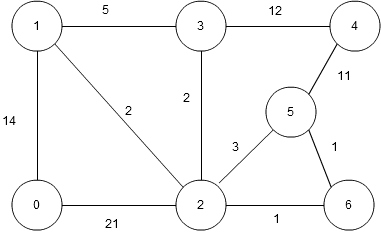
\includegraphics[scale=.7]{imgs/schema1.png}
\end{figure}

L'arbre couvrant minimum obtenu a un poids total de 31 :\\

\begin{figure}[h]
\centering
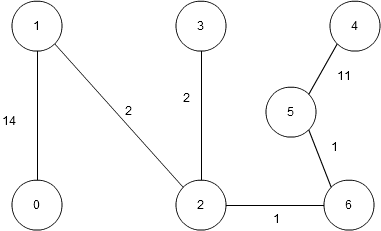
\includegraphics[scale=.7]{imgs/schema2.png}
\end{figure}

\clearpage
\subsection{Prim}

L'algorithme de {\bf Prim} permet également de résoudre le problème de l'arbre couvrant minimum. \\ 

Il s'agit ici de commencer avec un arbre contenant un seul sommet du graphe d'entrée, et à chaque tour ajouter un sommet. Le sommet choisi est celui qui est relié à un des sommets déjà ajouté (à l'arbre) avec l'arête de poids minimum. \\ 

Dans notre implémentation, nous avons choisi d'utiliser un vecteur d'arête trié par ordre croissant de la même manière que pour {\bf Kurskal} puisqu'il nous faut également filtrer les arêtes (graphe non-orienté). \\

Le graphe d'exemple pour cet algorithme est le même que pour l'algorithme de {\bf Kurskal} ({\it "minCoverTree.g"}). Les résultats sont donc identiques. \\

\clearpage
\section{Calcul du plus court chemin}
\subsection{Djikstra}
\subsubsection{L'algorithme :}

L'algorithme de {\bf Djikstra} permet de trouver le plus court chemin pour accéder à chaque sommet d'un graphe pondéré par des valeurs positives\footnote{L'utilisation d'une map a également un intérêt au niveau de la souplesse du template. En effet, utiliser un vecteur d'une taille égale au nombre de sommets du graphe impose que le type {\it vertex\_t} du graphe soit un type intégral afin qu'il puisse être utilisé en tant qu'indice de vecteur, ce qu'un conteneur associatif comme std$::$map n'impose pas.
Nous utilisons cependant des vecteurs de {\it vertex\_t} à d'autres endroit par soucis de simplicité.}. \\

Notre implémentation se base sur un principe d'incertitude. Dans un premier temps on ajoute le sommet d'origine comme sommet incertain (en réalité, la distance à l'origine du sommet d'origine est certaine, mais le premier cela permet de démarrer simplement l'algorithme). \\

A chaque tour de boucle, on choisit un sommet incertain S, qu'on marque alors comme certain. Pour chacun de ses successeurs T, on va calculer la distance à l'origine de I en passant par S, c’est-à-dire la distance à l'origine de S déjà calculée plus la valeur de l'arête (S, T). Si cette distance est inférieure à celle déjà calculée pour I, alors on met à jour la distance de I et I est marqué comme incertain. En effet, puisque la distance à l'origine de T a changé, il faut recalculer les distances à l'origine de tous les sommets pouvant avoir un chemin passant par T. \\

L'algorithme s'arrête lorsque plus aucun sommet n'est marqué comme incertain. Pour les graphes non fortement connexes, les sommets qui ne sont pas accessibles\footnote{En d'autres termes, les sommets qui ne sont pas successeurs du sommet d'origine dans le graphe transitif de G.} depuis l'origine auront une distance infinie (ils ne sont pas présent dans la map). \\

{\bf Djikstra} permet de trouver la distance minimale à l'origine de chaque sommet du graphe, mais également le chemin à parcourir pour obtenir cette distance minimale. \\

Pour ne pas perdre cette information, deux données sont stockée pour chaque sommet S : la distance minimale à l'origine et le sommet précédant S\footnote{On considère arbitrairement que le sommet d'origine a pour prédécesseur lui-même. Cette valeur est de toute façon inutile (et donc ignorée dans le code client) et nous permet d'éviter de manipuler des types autorisant une valeur nulle comme des pointeurs.}  dans le chemin pour atteindre S depuis l'origine. \\
\clearpage
De cette manière, on peut facilement retrouver le chemin pour atteindre le sommet S en remontant le chemin depuis S jusqu'à l'origine en regardant le sommet T précédant S, puis le sommet précédant T etc… jusqu'à retrouver l'origine.  \\

\subsubsection{Exemple :}
Le graphe d'exemple utilisé pour l'algorithme de {bf Djikstra} est contenu dans le fichier {\it "shortestPath.g"} :\\ 

\begin{figure}[h]
\centering
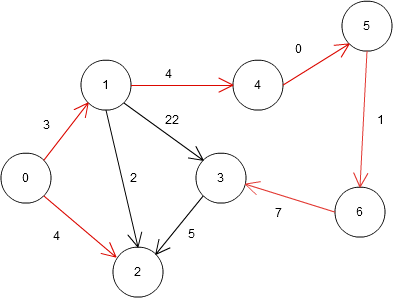
\includegraphics[scale=.8]{imgs/schema3.png}
\end{figure}

Nous avons ici coloré les arêtes des chemins utilisés pour atteindre les différents sommets depuis le sommet d'origine qui est ici le sommet 0. Par exemple, le plus court chemin pour atteindre le sommet 3 depuis 0 a un poids total de 15 et passe par les sommets 0, 1, 4, 5, 6 et enfin 3. \\
On peut constater que le graphe partiel de G comportant uniquement les arêtes colorés forme un équivalent d'un arbre couvrant de poids minimum pour les graphes orientés (bien que ce graphe partiel ne soit pas fortement connexe, donc la comparaison s'arrête ici). \\

\clearpage
\subsection{Bellman-Ford}
\subsubsection{L'algorithme :}
L'algorithme de {\bf Bellman-Ford} permet également d'obtenir le plus court chemin entre un sommet d'un graphe orienté et pondéré et tous les autres sommets. A la différence de l'algorithme de {\bf Djikstra}, il est capable de détecter les cycles d'absorption et donc de s'appliquer sur des graphes possédants des arêtes de poids négatif.
Comme pour {\bf Djikstra}, on commence par définir la distance à l'origine de chaque sommet à +infini (également traduit par une absence dans la map dans notre implémentation) excepté pour l'origine qui est à une distance de 0. \\

On va ensuite effectuer une boucle allant de 1 à |E| - 1 (où |E| est le nombre de sommets du graphe). Le tour n consistera à tester les chemins de longueur n depuis l'origine. Si un chemin a un poids total inférieur à la distance assigné au sommet d'arrivée, on met à jour la distance de ce sommet.
On effectue un tour de boucle supplémentaire. Si aucune distance n'est modifiée, alors le résultat est trouvé. Si au contraire une distance a diminué, c'est que le graphe comporte un cycle d'absorption. \\

Dans notre implémentation, nous avons choisi de retourner un tableau contenant les distances de chaque sommet à chaque étape (plutôt que de retourner une paire (distance, prédécesseur) comme pour {\bf Djikstra}) afin de mieux illustrer le fonctionnement de l'algorithme. \\

\subsubsection{Exemple :}

Le premier exemple pour l'algorithme est le même que pour l'algorithme de {\bf Djikstra} et fourni donc les même résultats. Dans un second temps, nous avons modifié ce graphe en ajoutant un cycle d'absorption. Ce graphe modifié est contenu dans le fichier {\it "shortestPathNegativeWeightCycle.g"} :\\ 

L'algorithme détecte bien la présence d'un cycle d'absorption (qui est ici coloré en vert sur le schéma).
Nous avons également coloré en rouge, le seul chemin minimum valide, qui relie le sommet 0 et le sommet 1. En effet, le sommet 1 est le seul sommet accessible depuis l'origine mais pas depuis un sommet appartenant au cycle d'absorption. Pour tous les autres sommets, plus on effectue de passage dans le cycle d'absorption, plus le poids du chemin les reliant à l'origine est petit.\\

\clearpage

\begin{figure}[h]
\centering
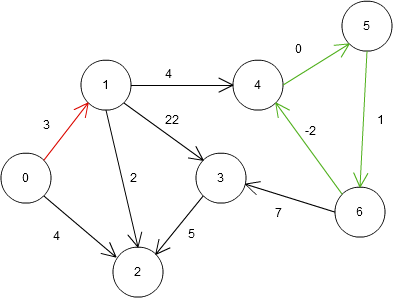
\includegraphics[scale=.7]{imgs/schema4.png}
\end{figure}

En revanche, l'algorithme de {\bf Bellman-Ford} ne permet pas de déterminer quels sont les chemins depuis l'origine dont le résultat est valide malgré le cycle d'absorption (en l'occurrence uniquement le sommet 1). Une solution serait de ré-appliquer l'algorithme de {\bf Bellman-Ford} sur des sous-graphes de G afin de déterminer le ou les cycles d'absorption et d'isoler les sommets qui ne sont pas concernés par celui(ceux)-ci.\\

\clearpage
\section{Welsh-Powell: coloration de graphe}
\subsubsection{L'algorithme :}
L'algorithme de {\bf Welsh-Powell} est un algorithme permettant la coloration de graphe non-orienté. La coloration de graphe consiste à attribuer une couleur (représentée par un {\it unsigned} ici) à chaque sommet, de manière à ce que deux sommets adjacents n'aient pas la même couleur.\\

Dans un premier temps, les sommets sont triés par degré (nombre de voisins). Ensuite, on effectue une boucle qui s'arrête lorsque tous les sommets sont colorés.\\ 
 A chaque tour de boucle on affecte une nouvelle couleur à un sommet non-encore coloré. On parcourt tous les autres sommets non-colorés et on leur affecte cette même couleur si et seulement si ils ne sont voisins avec aucun des sommets partageant cette couleur.\\
 
L'algorithme de {\bf Welsh-Powell} ne donne pas une coloration optimale. Notons que le tri par degré n'est pas indispensable pour obtenir une coloration, mais permet d'avoir une meilleure coloration dans le cas moyen.\\

\subsubsection{Exemple :}

Le premier graphe d'exemple pour l'algorithme de {\bf Welsh-Powell} est le suivant (coloration.g), coloré suivant le résultat de l'exécution de notre implémentation de l'algorithme :\\


\begin{figure}[h]
\centering
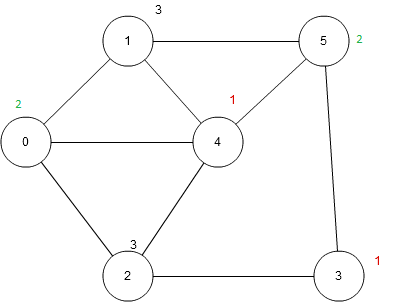
\includegraphics[scale=1.25]{imgs/schema5.png}
\end{figure}

L'algorithme de Welsh-Powell ne donne pas forcément la coloration optimale (c’est-à-dire la coloration utilisant le moins de couleur possible). La coloration fournie dépends du tri des sommets par leurs degrés (et de la position des sommets de degré équivalents dans la liste triée obtenu).\\

Un cas classique de divergence de résultat suivant le tri est la couronne à n-sommets (avec n un entier pair) dont la coloration optimale (nombre chromatique) est de 2 et qui a la particularité d'avoir un degré égal pour chaque sommet (et donc d'être très dépendant du tri). Pour illustrer ce phénomène nous avons utilisé une couronne à 8 sommets (graphe hexaédrique).\\

Ce graphe est stocké dans les fichiers {\it hexaédrique\_1.g} et {\it hexaédrique\_2.g} mais avec une numérotation des sommets différente. \\

Pour le premier fichier, la numérotation est optimale, et on obtient une coloration avec deux couleurs :\\ \\

\begin{figure}[h]
\centering
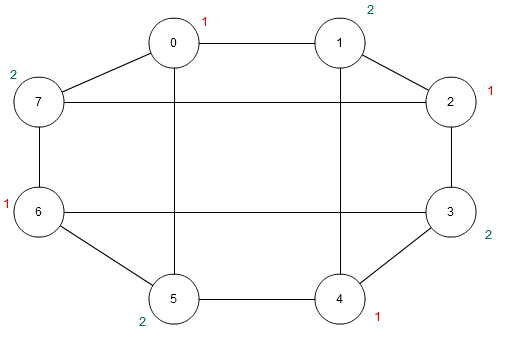
\includegraphics[scale=.7]{imgs/schema6.png}
\end{figure}

\clearpage
Pour la seconde en revanche, l'algorithme donne un nombre chromatique de 3, ce qui est incorrect :\\

\begin{figure}[h]
\centering
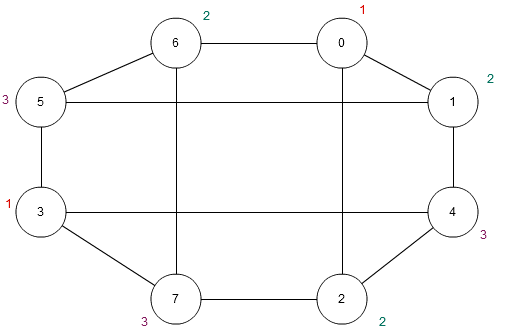
\includegraphics[scale=.7]{imgs/schema7.png}
\end{figure}
On peut emmètre l'hypothèse qu'il est possible de remplir le fichier (et donc de choisir la numérotation des sommets) d'un graphe de façon à ce que la coloration soit optimale et ce dès lors qu'on connait l'algorithme de tri utilisé (en particulier sa stabilité).\\

% REFERENCES 

\clearpage
\section{Références}
Pour notre projet, nous nous sommes inspirés des ressources suivantes : \\ 
\begin{itemize}
\item \href{https://isocpp.org/}{https://isocpp.org/} 
\item \href{http://cppreference.com}{http://cppreference.com}
\item \href{http://stackoverflow.com}{http://stackoverflow.com}
\item \href{https://msdn.microsoft.com}{https://msdn.microsoft.com} 
\item \href{https://openclassrooms.com}{https://openclassrooms.com}
\item \href{http://www.qtfr.org/}{http://www.qtfr.org/}
\item \href{http://cpp.developpez.com}{http://cpp.developpez.com}
\item \href{https://fr.wikipedia.org/wiki/Coloration_de_graphe#Algorithme_de_Welsh_et_Powell}{https://fr.wikipedia.org/wiki/Coloration\_de\_graphe\#Algorithme\_de\_Welsh\_et\_Powell}  \\
\end{itemize}

Le projet ne comporte pas de morceaux de code récupérés sur internet et n'utilise aucune bibliothèque tierce. \\
\end{document}